\documentclass[11pt]{article}
\usepackage{fullpage}
\usepackage{graphicx}
\usepackage{fourier}
\usepackage{xspace}
\usepackage{booktabs}
\usepackage{wrapfig}

\title{Assignment 1: \emph{Write Up}}
\author{Sriramya Prayaga}
\date{\today}

\begin{document}\maketitle

In this document, I'll be discussing the process of obtaining my graphs and
the results.
 
\section{Graph 1: Length}

For the length graph, other than echo, I only used the wc -l command. Because
this command counts the number of new lines, it was useful to determine how
many values of the Collatz sequence are in my data file --as, the collatz.c
program produces each value of a sequence on a new line. I used both echo and 
file redirection to output the sequence length results to a data file.

The graph appears to be an arch shape. The graph starts with multiple arch-like
curves that tend to flatten out as the value of 'n' increases. As can be seen
from the image, many adjacent values of n appear to have the same length. 

\begin{figure}[tbp]
\begin{centering}
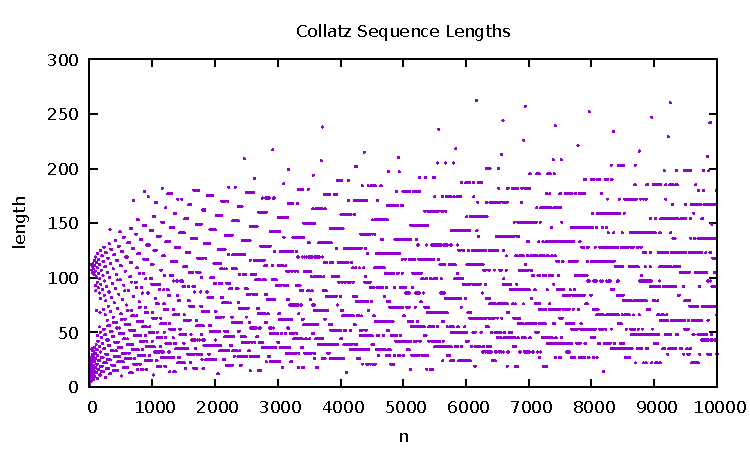
\includegraphics[width=0.75\textwidth]{CollatzSequenceLengths.pdf}
\caption {Length Graph}
\end{centering}
\end{figure}

\end{Graph 1: Length}

\section{Graph 2: Maximum Value}

For the maximum value graph, (other than echo) I used the sort -nr and head -n 1
commands. Because collatz.c produces output numbers that are unsorted, it was
necessary to numerically sort the values reversely in order to be able to extract
the value on the first line (which would be the greatest value, since the data
file is sorted.) I, once again, used pipes to output the result of sort -nr into
the command head -n 1.

The graph appears to have many trends. For instance, for many values of n, the graph
reveals that some frequent maximum values are 10000, 40000, and 80000. The graph also
reveals that for many other increasing values of n, the maximum value is also
linearly increasing. In fact, there are many positively sloped lines in the output
graph.

\begin{figure}[tbp]
\begin{centering}
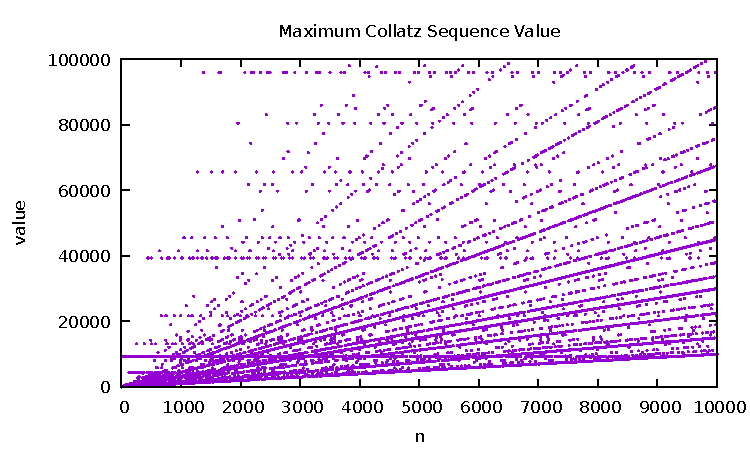
\includegraphics[width=0.75\textwidth]{MaximumCollatzSequenceValue.pdf}
\caption {Maximum Value Graph}
\end{centering}
\end{figure}

\end{Graph 2: Maximum Value}

\section{Graph 3: Length Frequency Histogram}

For the sequence length histogram, I used the awk, sort -n and uniq -c commands.
As I already had the sequence length data file generated for graph 1, I needed to
just get the second column of data in that file using awk. Then I needed to sort 
the data so that I can get all of the lengths of each n on an adjacent new line.
This is because if I want to use uniq -c to count the frequency of the lengths, the
data has to be on adjacent lines. Therefore, once I sorted all of the data, I would
be able to use uniq -c and get all of the frequencies of the lengths. 

The histogram reveals that the maximum frequency is 190 and occurs at length 53.
The graph also reveals that the lowest frequency is 1, of which many lengths have a
corresponding value. Something to note is that the frequencies of the lengths fluctuate
quite a bit. Usually, a length with a high frequency is followed by a length with a lower
corresponding frequency.

\begin{figure}[tbp]
\begin{centering}
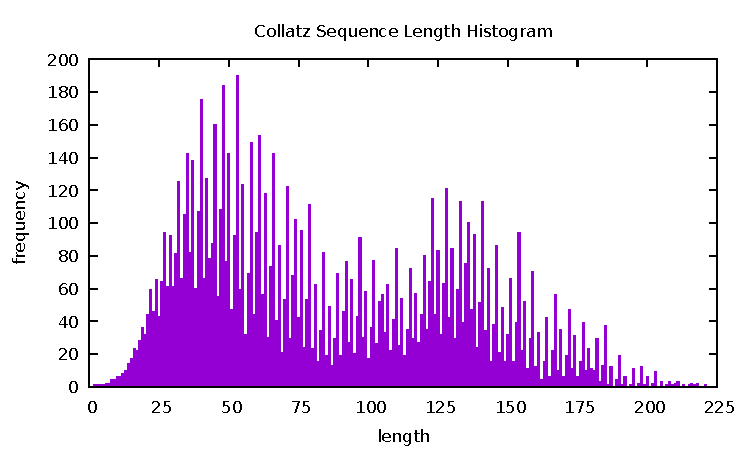
\includegraphics[width=0.75\textwidth]{CollatzSequenceLengthHistogram.pdf}
\caption {Length Frequency Histogram}
\end{centering}
\end{figure}

\end{Graph 3: Length Frequency Histogram}

\section{Graph 4: Random Collatz Lengths}

For my fourth graph, I used the same Unix commands I used to generate the first graph.
But, as collatz.c is dependent on the current time for its seed, and I wanted to
randomly run collatz.c, I had to use the additional command sleep 1 to pause the
computer for a second (so a new seed would be generated.)

Because it generates random results, the plot produces different results each time I run 
the program. However, a general tendency I've noticed with the graph results is that, when
run randomly 100 times, there usually tend to be clusters of data points at certain lengths.

\begin{figure}[tbp]
\begin{centering}
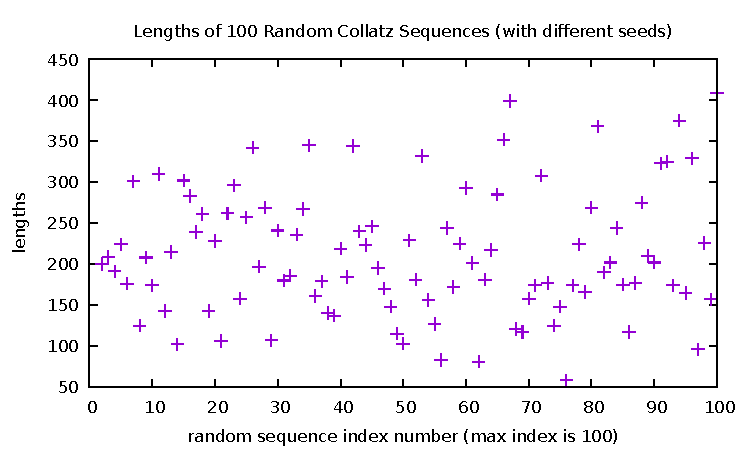
\includegraphics[width=0.75\textwidth]{randcollatz.pdf}
\caption {Lengths of Random Collatz Sequences}
\end{centering}
\end{figure}

\end{Graph 4: Random Collatz Lengths}

\section{What I Learned}       

Overall, it can be noted that these graphs have certain trends for certain 
values of n, but behave differently when there are other values of n. 

In order to achieve these results and observe these graphs, I had to make
many modifications to my code and learned some valuable information about
bash scripts.

To be clear, as this was my first time writing control structures in bash,
I had originally made many syntax errors while trying to output the length plot.
For example, I would forget to include keywords like done and fi often. However,
once I got the hang of it, it became easier to focus on other aspects of the
assignment (like utilizing the Unix commands to generate data.)

Another issue I had originally was my code took a long time to run. To be              
clear, the third graph that we had to plot (the frequency of the lengths
graph), took up more time than it should because I wrote a for-loop to count the
sequence lengths again. However, as I already had this data generated from the
first graph, it was an unnecessary thing to do. Once I used my previous data file, 
my code ran around 20 seconds faster.
\end{What I learned}



\end{document}


